% !TEX root = Thesis.tex
\chapter{Introduction}\label{chap:Intro}

  This is the Introduction in the dissertation. Here is an example of reference journal or transaction ~\cite{msc-bhattacharya-tcad06}

  \section{Overview}\label{sec:overview}

    Section Here

    \subsection{Analog circuit synthesis with performance exploration}\label{subsec:PAGEOverview}

      Subsection Here. Here is the example of single picture in Figure~\ref{fig:OverallFlow}

      \begin{figure}[ht]
        \centerline{
        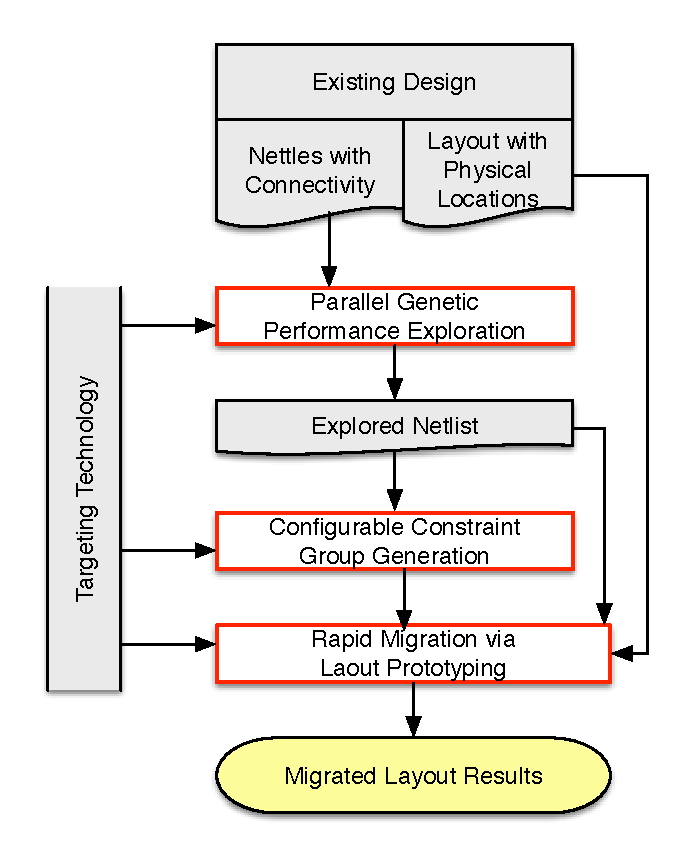
\includegraphics[width=0.6\textwidth]{Fig/Introduction/OverallFlow.eps}}
        \caption{The overall flow} 
        \label{fig:OverallFlow}
      \end{figure}

      \subsubsection{Previous Works}
        
        Multiple subfigure is shown in Figure~\ref{fig:RoutingPreserv}. On of subfigure is ~\ref{fig:RoutingPreserv_A}

      \begin{figure}
        \centering
        \begin{subfigure}[t]{0.4\textwidth}
        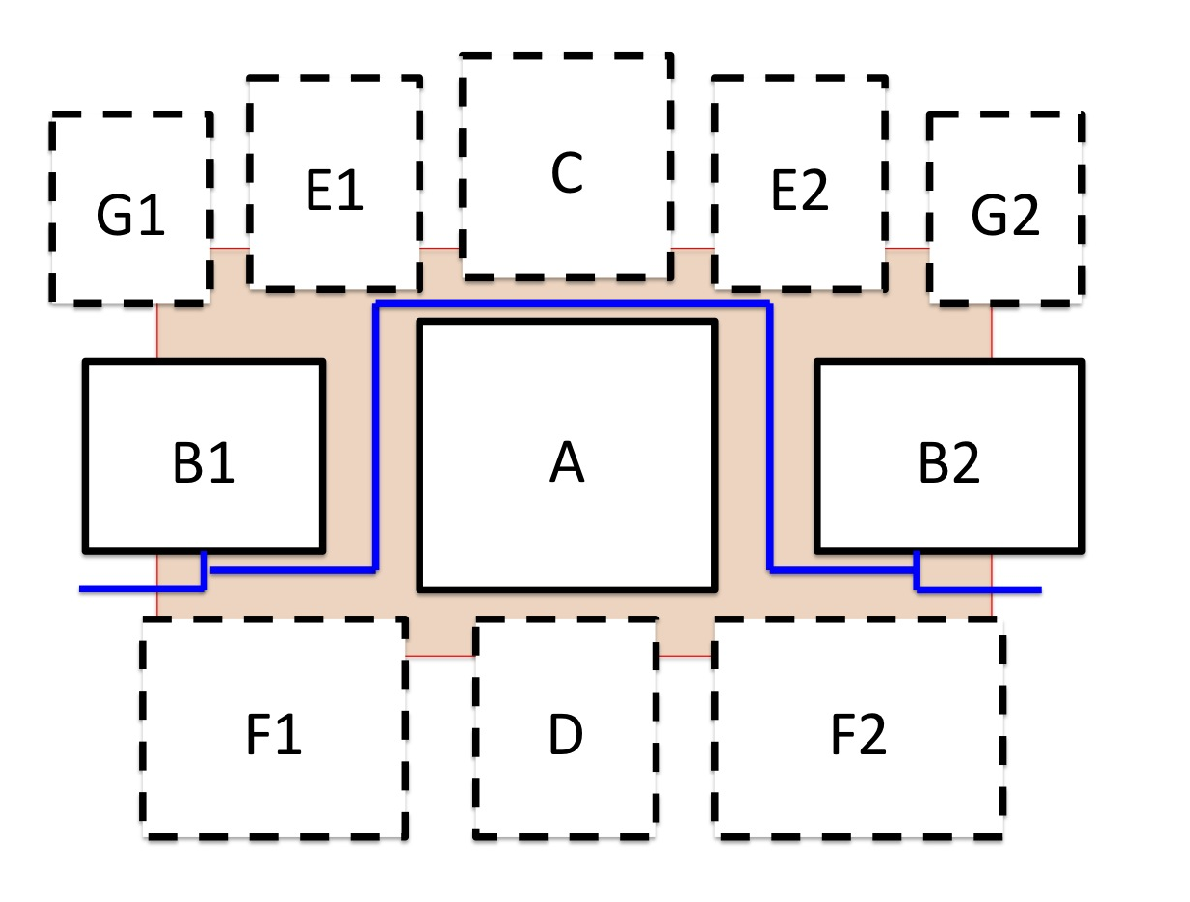
\includegraphics[width=\textwidth]{Fig/Introduction/RoutingPreserv_a.eps}
        \caption{Reference template layout}
        \label{fig:RoutingPreserv_A}
        \end{subfigure}
        \begin{subfigure}[t]{0.4\textwidth}
        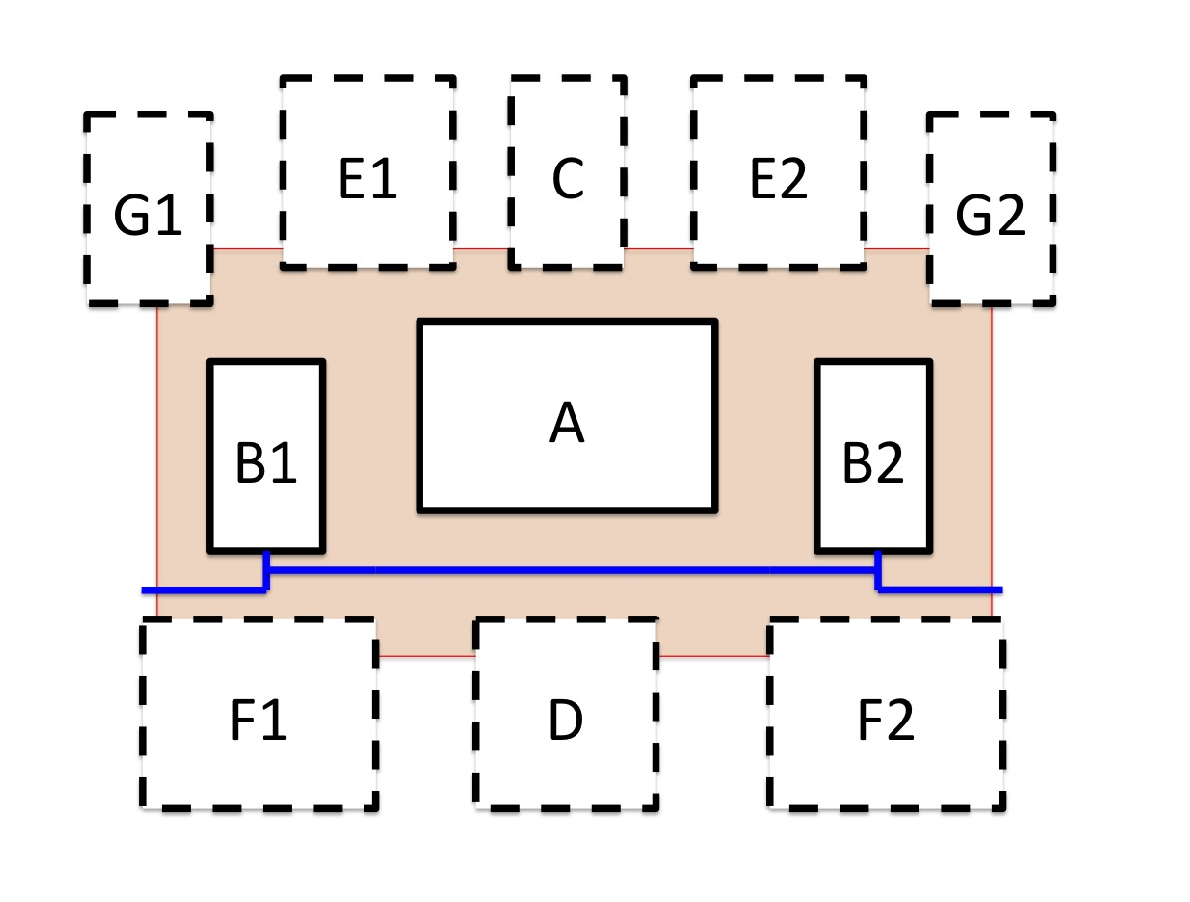
\includegraphics[width=\textwidth]{Fig/Introduction/RoutingPreserv_b.eps}
        \caption{Non-preserved automatic routing}
        \label{fig:RoutingPreserv_B}
        \end{subfigure}
        \begin{subfigure}[t]{0.4\textwidth}
        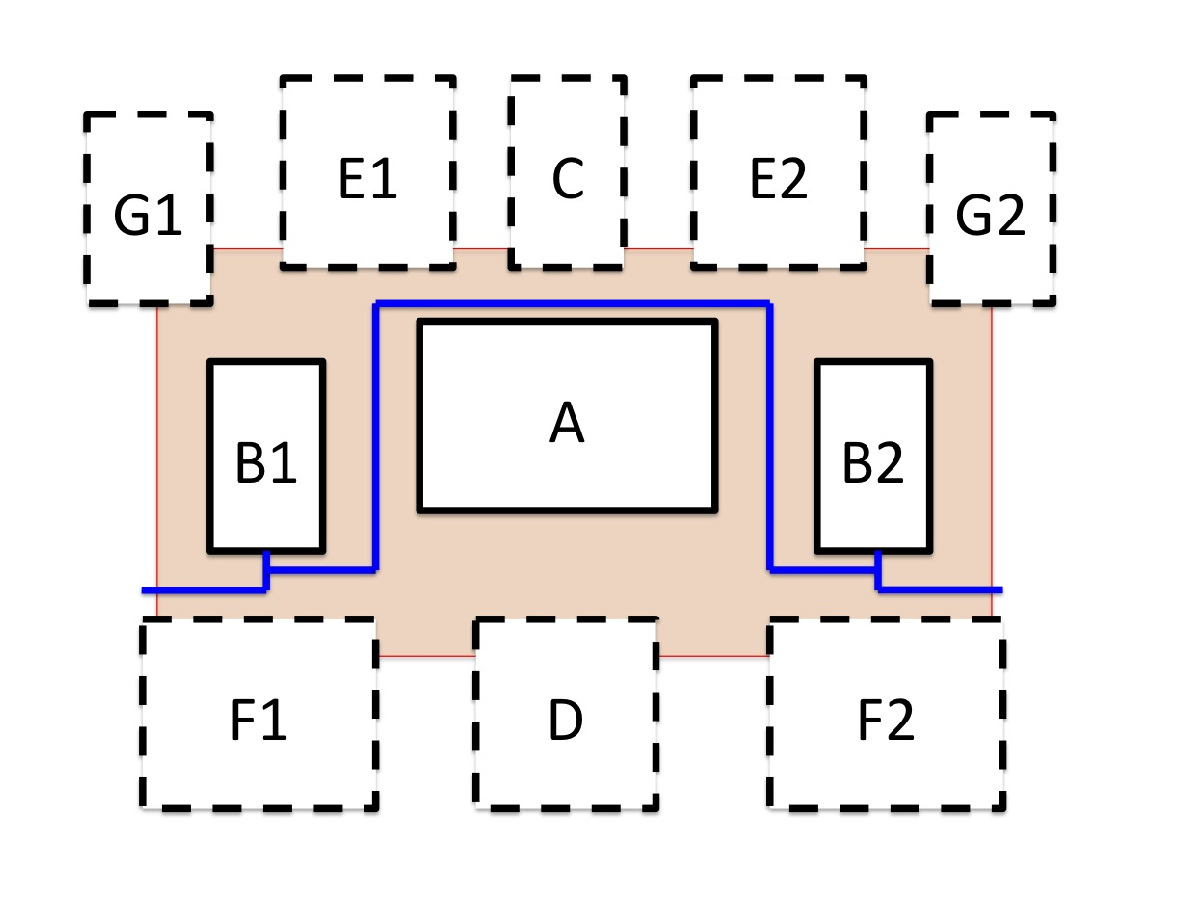
\includegraphics[width=\textwidth]{Fig/Introduction/RoutingPreserv_c.eps}
        \caption{Preserved routing}
        \label{fig:RoutingPreserv_C}
        \end{subfigure}
        \begin{subfigure}[t]{0.4\textwidth}
        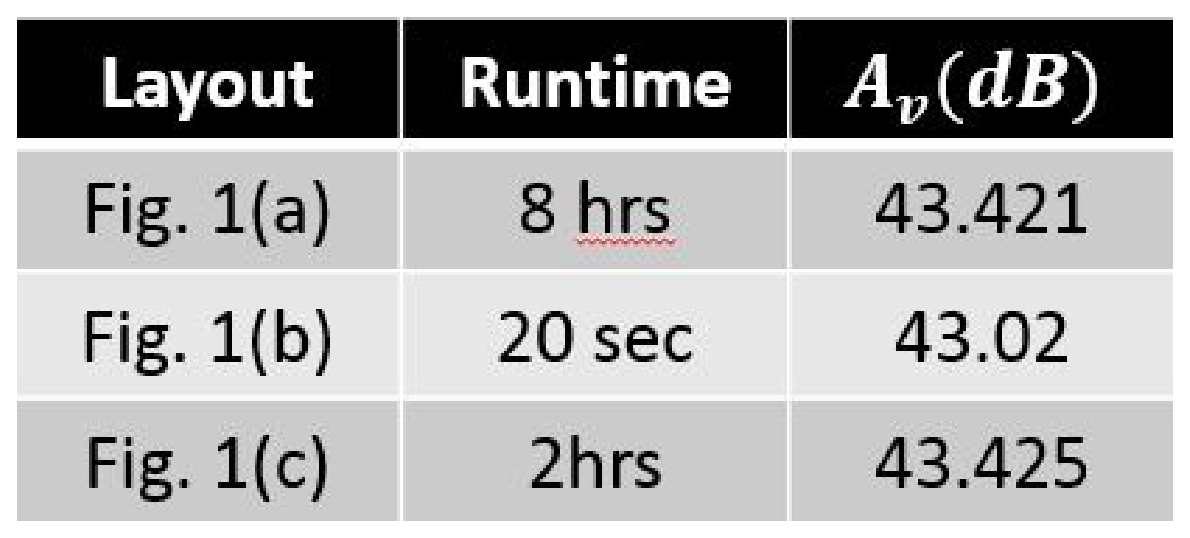
\includegraphics[width=\textwidth]{Fig/Introduction/RoutingPreserv_d.eps}
        \caption{Timing and simulation results}
        \label{fig:RoutingPreserv_d}
        \end{subfigure}
        \caption{Analog layout generation with different configuration. (a) Reference layout with complete placement and routing. (b) Non-preserved automatic routing considering usual constraints only. (c) Layout generation considering preserved routing characteristics. (d) Simulation results in umc65nm technology.}
        \label{fig:RoutingPreserv}
      \end{figure}

